%%%%%%%%%%%%%%%%%%%%%%%%%%%%%%%%%%%%%%%%%%%%%%%%%%%%%%%%%%%%%%%%%%%%%%%%%%%%%%%%
%
% Template license:
% CC BY-NC-SA 3.0 (http://creativecommons.org/licenses/by-nc-sa/3.0/)
%
%%%%%%%%%%%%%%%%%%%%%%%%%%%%%%%%%%%%%%%%%%%%%%%%%%%%%%%%%%%%%%%%%%%%%%%%%%%%%%%%

%----------------------------------------------------------------------------------------
%	PACKAGES AND OTHER DOCUMENT CONFIGURATIONS
%----------------------------------------------------------------------------------------
\documentclass[
11pt, % The default document font size, options: 10pt, 11pt, 12pt
%oneside, % Two side (alternating margins) for binding by default, uncomment to switch to one side
%chapterinoneline,% Have the chapter title next to the number in one single line
spanish,
singlespacing, % Single line spacing, alternatives: onehalfspacing or doublespacing
%draft, % Uncomment to enable draft mode (no pictures, no links, overfull hboxes indicated)
%nolistspacing, % If the document is onehalfspacing or doublespacing, uncomment this to set spacing in lists to single
%liststotoc, % Uncomment to add the list of figures/tables/etc to the table of contents
%toctotoc, % Uncomment to add the main table of contents to the table of contents
parskip, % Uncomment to add space between paragraphs
%codirector, % Uncomment to add a codirector to the title page
headsepline, % Uncomment to get a line under the header
]{MastersDoctoralThesis} % The class file specifying the document structure

\usepackage{subcaption}
\usepackage{gensymb}
\usepackage[backend=bibtex,
			natbib=true,
			style=numeric,
			sorting=none]
{biblatex}

%----------------------------------------------------------------------------------------
%	INFORMACIÓN DE LA MEMORIA
%----------------------------------------------------------------------------------------

\thesistitle{Adquisidor y display en tiempo real de datos de motores de combustión interna} % El títulos de la memoria, se usa en la carátula y se puede usar el cualquier lugar del documento con el comando \ttitle

% Nombre del posgrado, se usa en la carátula y se puede usar el cualquier lugar del documento con el comando \degreename
\posgrado{Carrera de Especialización en Sistemas Embebidos} 
%\posgrado{Carrera de Especialización en Internet de las Cosas} 
%\posgrado{Carrera de Especialización en Intelegencia Artificial}
%\posgrado{Maestría en Sistemas Embebidos} 
%\posgrado{Maestría en Internet de las cosas}

\author{Ing. Ignacio Moya} % Tu nombre, se usa en la carátula y se puede usar el cualquier lugar del documento con el comando \authorname

\director{Mg. Ing. Tomás Porreca (IUA ; FAA)} % El nombre del director, se usa en la carátula y se puede usar el cualquier lugar del documento con el comando \dirname
\codirector{Nombre del codirector (pertenencia)} % El nombre del codirector si lo hubiera, se usa en la carátula y se puede usar el cualquier lugar del documento con el comando \codirname.  Para activar este campo se debe descomentar la opción "codirector" en el comando \documentclass, línea 23.

\juradoUNO{Esp. Ing. Gonzalo Daniel Sánchez (FIUBA)} % Nombre y pertenencia del un jurado se usa en la carátula y se puede usar el cualquier lugar del documento con el comando \jur1name
\juradoDOS{Ing. Yanina Dinora Menchón (FCEIA-UNR)} % Nombre y pertenencia del un jurado se usa en la carátula y se puede usar el cualquier lugar del documento con el comando \jur2name
\juradoTRES{Mg. Ing. Pablo Slavkin (FIUBA)} % Nombre y pertenencia del un jurado se usa en la carátula y se puede usar el cualquier lugar del documento con el comando \jur3name

%\ciudad{Ciudad Autónoma de Buenos Aires}
\ciudad{ciudad de Rosario}

\fechaINICIO{octubre de 2020}
\fechaFINAL{octubre de 2023}


\keywords{Sistemas embebidos, FIUBA} % Keywords for your thesis, print it elsewhere with \keywordnames


\begin{document}


\frontmatter % Use roman page numbering style (i, ii, iii, iv...) for the pre-content pages

\pagestyle{plain} % Default to the plain heading style until the thesis style is called for the body content


%----------------------------------------------------------------------------------------
%	RESUMEN - ABSTRACT 
%----------------------------------------------------------------------------------------

\begin{abstract}
\addchaptertocentry{\abstractname} % Add the abstract to the table of contents
%
%The Thesis Abstract is written here (and usually kept to just this page). The page is kept centered vertically so can expand into the blank space above the title too\ldots
\centering

Esta memoria describe el proceso realizado para diseñar e implementar un adquisidor y display en tiempo real de datos de motores de combustión interna. El sistema de desarrolló con el propósito de brindar a vehículos antiguos funcionalidades que se encuentran solo en vehículos modernos, y darle al usuario información útil sobre el funcionamiento interno de su máquina para ser usada en su mantenimiento o puesta a punto.
El trabajo se realizó como parte de un emprendimiento propio.
Para este trabajo fueron fundamentales conocimientos sobre ingeniería de software, sistemas operativos en tiempo real, protocolos de comunicación para sistemas embebidos y diseño de circuitos impresos.

\end{abstract}

%----------------------------------------------------------------------------------------
%	CONTENIDO DE LA MEMORIA  - AGRADECIMIENTOS
%----------------------------------------------------------------------------------------

\begin{acknowledgements}
%\addchaptertocentry{\acknowledgementname} % Descomentando esta línea se puede agregar los agradecimientos al índice
\vspace{1.5cm}

Esta sección es para agradecimientos personales y es totalmente \textbf{OPCIONAL}.  

\end{acknowledgements}

%----------------------------------------------------------------------------------------
%	LISTA DE CONTENIDOS/FIGURAS/TABLAS
%----------------------------------------------------------------------------------------

\tableofcontents % Prints the main table of contents

\listoffigures % Prints the list of figures

\listoftables % Prints the list of tables


%----------------------------------------------------------------------------------------
%	CONTENIDO DE LA MEMORIA  - DEDICATORIA
%----------------------------------------------------------------------------------------

% \dedicatory{\textbf{Dedicado a... [OPCIONAL]}}  % escribir acá si se desea una dedicatoria

%----------------------------------------------------------------------------------------
%	CONTENIDO DE LA MEMORIA  - CAPÍTULOS
%----------------------------------------------------------------------------------------

\mainmatter % Begin numeric (1,2,3...) page numbering

\pagestyle{thesis} % Return the page headers back to the "thesis" style

% Incluir los capítulos como archivos separados desde la carpeta Chapters

% Chapter 1

\chapter{Introducción general} % Main chapter title

Este capitulo explica los motivos detrás de la decisión de realizar este trabajo final. Realiza una comparación entre el dispositivo desarrollado y productos de características similares que están disponibles en el mercado. Y finalmente enumera los alcances y objetivos del trabajo final.

\label{Chapter1} % For referencing the chapter elsewhere, use \ref{Chapter1} 
\label{IntroGeneral}

%----------------------------------------------------------------------------------------

% Define some commands to keep the formatting separated from the content 
\newcommand{\keyword}[1]{\textbf{#1}}
\newcommand{\tabhead}[1]{\textbf{#1}}
\newcommand{\code}[1]{\texttt{#1}}
\newcommand{\file}[1]{\texttt{\bfseries#1}}
\newcommand{\option}[1]{\texttt{\itshape#1}}
\newcommand{\grados}{$^{\circ}$}

%----------------------------------------------------------------------------------------

%\section{Introducción}

%----------------------------------------------------------------------------------------
\section{Motivación}

Desde el año 1991 en adelante, todos los fabricantes de vehículos de combustión interna están obligados a incluir en sus vehículos un sistema electrónico de diagnóstico. Este sistema, conocido por sus siglas en inglés como OBD (On-Board Diagnostics), realiza las tareas de muestrear sensores que están conectados físicamente sobre el motor y alertar al conductor, a través de un indicador en el tablero, cuando el motor no está funcionando dentro de los parámetros de operación. También mantiene un registro interno de los fallos ocurridos durante la vida del mismo, para luego ser descargado por el mecánico encargado de realizar tareas de reparación o puesta a punto, y así facilitar su trabajo.
Actualmente existen grupos de entusiastas y coleccionistas que poseen vehículos fabricados antes de que el sistema OBD se haga obligatorio. Y por esa razón, no tienen la posibilidad de hacer un monitoreo del funcionamiento del motor de su vehículo. Tampoco es posible mantener un registro de si hubo eventos de fallas o momentos de operación fuera de rango, información útil para su mantenimiento preventivo.
Por esto es que se tomó la decisión de desarrollar para este Trabajo Final, un dispositivo que cumpla las mismas funciones que un OBD, pero para vehículos antiguos que no tienen instalado dicho sistema de fábrica.

\section{Estado del arte}

Comparación del sistema con productos similares del mercado.

\section{Alcance y objetivos}

Explicar que se pretende obtener finalizado el desarrollo.



\chapter{Introducción específica} % Main chapter title

\label{Chapter2}

En este capítulo se explica en detalle el funcionamiento de un motor de combustión interna y se describe el sistema de desarrollado, sus partes y la interacción entre ellas. Al final los requerimientos del proyecto.

\section{Funcionamiento de un motor de combustión interna} \label{func-motor}

En la actualidad, el motor de combustión interna es el motor más utilizado en vehículos de transporte de cargas y pasajeros. Existen distintos tipos de motores que utilizan distintos tipos de combustibles. En esta sección se explicará específicamente sobre el funcionamiento de motores de pistón a gasolina de cuatro tiempos. Los motores de pistón utilizan un mecanismo llamado cigüeñal para convertir el movimiento lineal que el pistón recorre dentro de la cámara de combustión en un movimiento rotatorio que finalmente se transmite a las ruedas del vehículo a través de una transmisión.

En dos revoluciones completas del cigüeñal el pistón pasa por cuatro etapas, representadas en la figura \ref{fig:motor-combustion}
\begin{itemize}
\item{Admisión:} Se ingresa a la cámara de combustión una mezcla de aire y combustible, gracias al movimiento hacia abajo del pistón que genera vacío dentro de la cámara.
\item{Compresión:} El pistón se mueve hacia arriba comprimiendo la mezcla de aire y combustible, con esto también aumenta su temperatura.
\item{Combustión:} A través de una chispa generada por una bujía se enciende la mezcla y se produce la combustión.
\item{Escape:} La combustión genera gases que son evacuados de la cámara por el movimiento hacia arriba del pistón. Luego de esta etapa final el proceso de repite y el pistón vuelve a la etapa de admisión.
\end{itemize}

\begin{figure}[htpb]
\centering
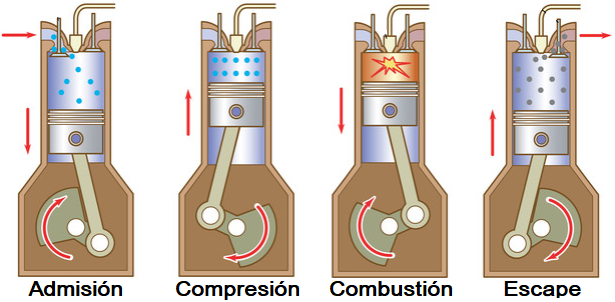
\includegraphics[width=.9\textwidth]{./Figures/motor-combustion.png}
\caption{Representación gráfica de las etapas de un motor de combustión de cuatro tiempos \protect\footnotemark[3].}
\label{fig:motor-combustion}
\end{figure}

\subsection{Proceso de combustión y su eficiencia}

Un motor de combustión interna, o motor a explosión, es un tipo de máquina que obtiene energía mecánica a través de una reacción química conocida como combustión. La combustión es la oxidación rápida en presencia de oxígeno de materiales llamados combustibles. El resultado de esta reacción, cuando la reacción es completa es, dióxido de carbono, agua, y energía liberada en forma de calor y expansión gaseosa. Es la energía liberada en forma de expansión gaseosa que es convertida en energía mecánica, y la energía liberada en forma de calor es disipada a la atmósfera. Cuando la combustión no es completa, ya sea por exceso o defecto de oxígeno, se producen otros compuestos parcialmente oxidados como el monóxido de carbono, cuando esto sucede la cantidad total de energía liberada es menor.

Para que una combustión sea completa se tiene que cumplir la condición de que la proporción por peso de oxígeno y combustible sea igual a su proporción estequiométrica. En un motor de gasolina esta proporción es de 14,7 partes de oxígeno por 1 parte de combustible \citep{book-afr}. Se le llama factor lambda, denominado con la letra griega $\lambda$, a la relación entre la proporción oxígeno y combustible actual con su proporción estequiométrica. Si la combustión ocurre con exceso de oxígeno el factor lambda será mayor a 1, si ocurre con defecto de oxígeno el factor será menor a 1, y si ocurre con la proporción justa será igual a 1. Los sensores desarrollados para poder monitorear este factor son llamados sondas lambda. En los vehículos actuales, el monitoreo de este factor es utilizado para regular la cantidad de combustible inyectada en cada proceso de combustión, de esa forma es posible operar al motor de forma eficiente minimizando las emisiones de gases indeseados.

Otra variable que afecta a la cantidad de combustible inyectada es la temperatura de los gases de admisión. La densidad de un gas depende de su temperatura y, como el volumen de la cámara de combustión es fijo, es posible calcular el peso total de oxígeno que puede caber dentro de la cámara y por lo tanto define la cantidad máxima de combustible que puede inyectarse. A menor temperatura del gas, su densidad aumenta y por lo tanto la cantidad de combustible que puede inyectarse para alcanzar la relación estequiométrica es mayor. Pero si la temperatura del gas es alta, la cantidad de combustible que puede inyectarse es menor y a menor cantidad de combustible la energía total entregada es menor.

\footnote[3]{Imagen tomada de \cite{motor}}

\subsection{Eficiencia mecánica y lubricación}

Sólo una parte de la energía mecánica proveniente del proceso de combustión es convertida en energía cinética. Parte de esa energía se pierde por la fricción entre las partes móviles que componen al motor. Para disminuir esta fricción se utilizan fluidos lubricantes, que funcionan impidiendo el contacto entre dos partes móviles. La fricción entre las partes móviles y el lubricante será menor que la fricción si las partes estuvieran en contacto, y al disminuir la fricción la energía perdida es menor. Para que el lubricante funcione adecuadamente su viscosidad tiene que estar dentro de un rango definido por el fabricante del motor, la misma es dependiente de la temperatura y por eso es importante monitorearla \cite{lubrication}. La temperatura de operación de un lubricante es indicada por su fabricante y su viscosidad es garantizada sólo dentro de ese margen de operación.

El lubricante es distribuido a las partes móviles del motor a través de un circuito hidráulico cerrado. Este circuito consiste de conductos, un tanque de almacenamiento y una bomba hidráulica. La operación de esta bomba garantiza la renovación del lubricante ya que parte del lubricante se pierde por el movimiento de las partes del motor y tiene que ser recolectado y devuelto al tanque de almacenamiento. Una presión hidráulica insuficiente puede ocasionar daños en el motor por falta de lubricación. Por eso la presión de aceite es monitoreada junto con la temperatura.

\subsection{Batería eléctrica}
Los motores no pueden operar sin una fuente de energía eléctrica ya que necesitan esta energía para dos procesos importantes: el arranque o puesta en marcha y la ignición del proceso de combustión.
Para arrancar un motor de combustión interna se utiliza un motor eléctrico que hace girar el cigüeñal y mueve al pistón por sus cuatro etapas. Una vez que se produce la combustión, la propia inercia del sistema hace que la operación sea sostenida. En aplicaciones móviles, el motor eléctrico es alimentado por una batería eléctrica, que por lo general son baterías de plomo y ácido con tensión nominal entre bornes de 12 V. Una tensión baja de la batería puede causar que el motor eléctrico no tenga suficiente torque para hacer girar el cigüeñal, o no pueda hacerlo girar a la velocidad suficiente para arrancarlo. Por otro lado, si la tensión de la batería disminuye demasiado al intentar arrancar un motor, esto puede indicar que la batería está descargada o que la fricción del motor es muy grande debido a fallas mecánicas o falta de lubricación.

La bujía que produce la chispa necesaria para iniciar la combustión también es alimentada a través de un circuito eléctrico por la batería del motor. Si la batería no tiene tensión suficiente, puede causar que la bujía no genere una chispa o que esta no sea suficiente para lograr la ignición de la mezcla de aire y combustible.

En un vehículo existen otros sub-sistemas que son alimentados por la batería del motor como: las luces, panel de información, sistema de audio, etc. Y todos ellos dependen de que la tensión de la batería se encuentre dentro de sus valores nominales para un correcto funcionamiento.

\section{Descripción general del sistema}

El sistema desarrolado consiste de dos partes distintas, la adquisidora de datos y la interfaz gráfica. La primer parte consiste de un circuito controlado por microprocesador montado cerca del motor del vehículo. El adquisidor digitaliza las señales producidas por los sensores de: temperatura de gases de admisión y escape; temperatura de aceite; sonda lambda; velocidad de giro; y tensión de la batería. Los sensores fueron seleccionados según el funcionamiento del motor explicado en \ref{func-motor}.  La información capturada por la parte adquisidora es transmitida a la segunda parte del sistema por \textit{Bluetooth Low-Energy}.

La interfaz está compuesta por una \textit{Single Board Computer}, una pantalla LCD táctil, y una tarjeta SD para almacenar los datos recibidos o puede ser un dispositivo móvil como un \textit{Smartphone} o \textit{Tablet}. La función de esta parte del sistema es de mostrar la información recibida en gráficas e indicar con alarmas visuales y sonoras cuando el valor de alguna de las variables es superior al límite establecido por el usuario. También almacena los datos recibidos en la memoria del dispositivo para luego descargar la información y analizarla posteriormente. Esta parte del sistema va ubicada en la cabina del vehículo en un lugar con fácil acceso y que sea visible por el conductor.

La figura \ref{fig:diagrama-de-bloques} es una representación en diagrama de bloques del sistema.

\begin{figure}[htpb]
\centering
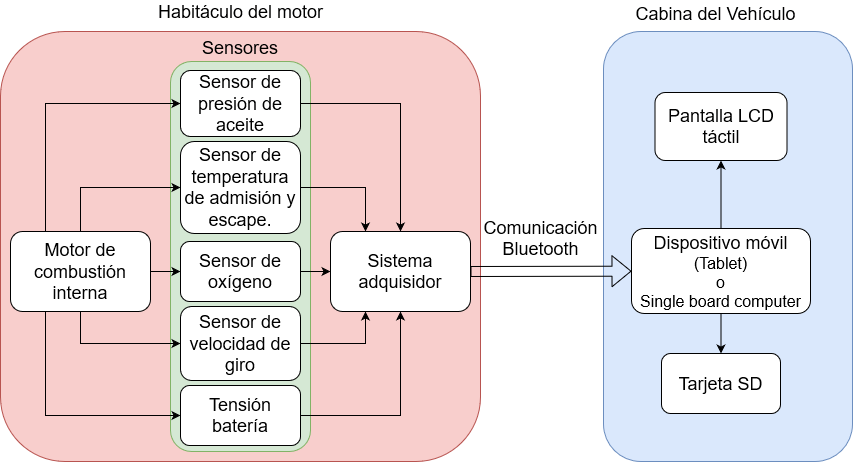
\includegraphics[width=.9\textwidth]{./Figures/diagrama-proyecto.png}
\caption{Diagrama en bloques del sistema.}
\label{fig:diagrama-de-bloques}
\end{figure}

\section{Requerimientos del proyecto}

El desarrollo del trabajo final fue basado en las historias de usuario y los requerimientos fijados durante la etapa de planificación del proyecto. Los requerimientos se dividieron en cuatro grupos: requerimientos generales del proyecto; requerimientos de la interfaz gráfica; requerimientos de la parte adquisidora de datos y requerimientos de la comunicación entre las partes.

Los requerimientos generales del proyecto son:
\begin{itemize}
\item REQ-GEN-001: todo el código fuente del proyecto será almacenado bajo un sistema de control de versiones GIT.
\item REQ-GEN-002: la documentación del código fuente del software embebidos será llevada a cabo en los comentarios, siguiendo el formato de Doxygen.
\item REQ-GEN-003: la documentación del software para la interfaz gráfica también será llevada a cabo en los comentarios. El formato será elegido por el responsable del proyecto.
\end{itemize}

Requerimientos de la interfaz gráfica:
\begin{itemize}
\item REQ-GUI-001: la interfaz gráfica deberá poder mostrar figuras con la información de todos los sensores a la vez.
\item REQ-GUI-002: el usuario tiene que poder elegir qué sensores ver al mismo tiempo y cuáles no desea ver.
\item REQ-GUI-003: el usuario tiene que poder definir alarmas por valor máximo, para cada una de las variables.
\item REQ-GUI-004: las alarmas serán sonoras y visuales. El estilo de las alarmas será definido por el cliente durante el proceso de desarrollo de la interfaz gráfica.
\end{itemize}

Requerimientos de la parte adquisidora:
\begin{itemize}
\item REQ-ADQ-001: el sistema tiene que adquirir la temperatura de los gases de admisión y escape, con un rango de temperatura entre 0 \degree C y 400 \degree C y con una resolución menor igual a 0,5 \degree C. Con una tasa de muestreo mayor o igual a 1 hz.
\item REQ-ADQ-002: el sistema tiene que adquirir la temperatura del aceite del motor, con un rango de temperatura entre 0 \degree C y 400 \degree C y una resolución menor igual a 0,5 \degree C. Con una tasa de muestreo mayor igual a 1 hz.
\item REQ-ADQ-003: el sistema tiene que adquirir la velocidad de giro del motor, en un rango entre 0 y 20.000 revoluciones por minuto, con una resolución menor igual a 500 r.p.m. Con una tasa de muestreo mayor igual a 5 hz.
\item REQ-ADQ-004: el sistema tiene que adquirir la proporción de oxígeno en los gases de escape llamada lambda, con un rango de 0 a 2 y una resolución menor igual a 0,1 lambda.
\item REQ-ADQ-005: el sistema tiene que adquirir la presión de aceite del motor, con un rango de 0 a 100 psi y con una resolución menor igual a 1 psi.
\item REQ-ADQ-006: el sistema debe comenzar a transmitir a la interfaz gráfica la información obtenida en un tiempo no mayor a 1 segundo transcurrido el proceso de adquisición.
\end{itemize}

Requerimientos de la comunicación entre las partes del sistema:
\begin{itemize}
\item REQ-COMM-001: se permitirá que se pierda hasta 1 paquete de cada 100 paquetes transmitidos.
\end{itemize} 
\chapter{Diseño e implementación} % Main chapter title

\label{Chapter3}

Este capítulo describe en detalle el sistema implementado, sus partes y su interacción, incluyendo los criterios adoptados durante el proceso de desarrollo. Luego, se explica qué sensores se utilizaron y su funcionamiento, qué componentes fueron utilizados para el circuito impreso. Y, finalmente, describe el funcionamiento y el proceso de desarrollo del software utilizado en la parte adquisidora y la interfaz gráfica.

\section{Desarrollo del circuito impreso} \label{circuito}

Para el prototipo se desarrolló un circuito impreso que funciona como "poncho"  para la EDU-CIAA. Un poncho es un circuito impreso con conectores específicos para conectarse a la EDU-CIAA y acceder a sus señales \cite{poncho}. El diseño se hizo con el software KiCAD versión 6. El circuito cumple las funciones de alimentación, digitalización de las señales de los sensores y comunicación con el módulo \textit{Bluetooth}. En la figura \ref{fig:circuito-3d} puede verse un renderizado del circuito finalizado. 

\begin{figure}[htpb]
\centering
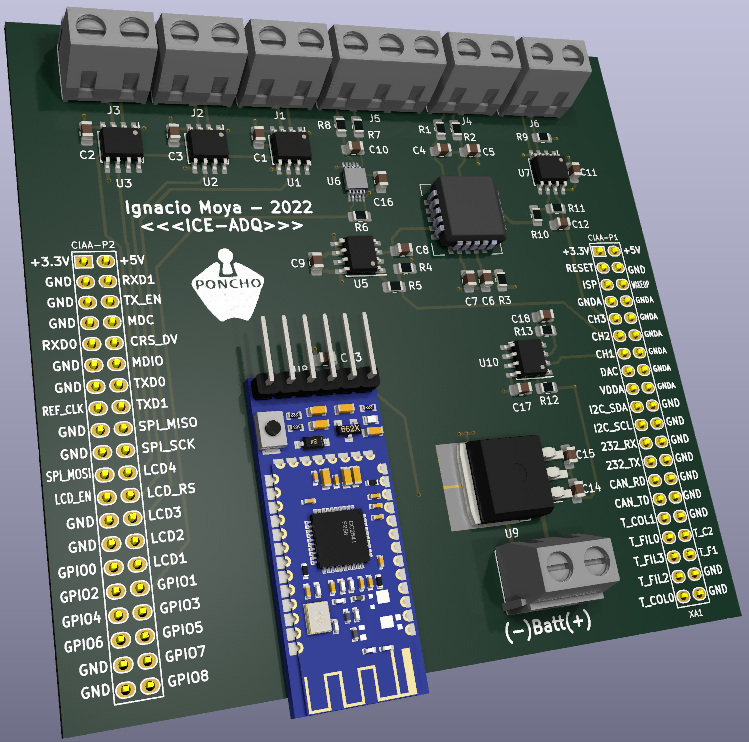
\includegraphics[width=.8\textwidth]{./Figures/circuito-3d.png}
\caption{Renderizado 3D del circuito finalizado.}
\label{fig:circuito-3d}
\end{figure}


\subsection{Circuito de medición de batería, oxígeno y presión de aceite}

Las variables analógicas son generadas por los sensores lambda, presión de aceite y la tensión de la batería. Para digitalizar estas señales se utilizó el conversor analógico digital de la ECU-CIAA, con sus tres canales independientes. Para esto fue necesario desarrollar tres circuitos amplificadores para llevar las señales producidas por los sensores, a señales de tensión dentro del rango de 0 V a 3,3 V. Y así hacer uso de el rango máximo del conversor analógico digital, que es de 10 bits. Para los circuitos amplificadores se utilizó el amplificador operacional LM358. Principalmente por su capacidad de poder tener una salida de 0 V cuando se lo alimenta con una fuente simple \cite{lm358}. Su salida puede llegar a 1,5 V por debajo de su tensión de alimentación. Por lo que al alimentarlo con una fuente de simple de 5V, su tensión de salida puede variar entre 0 V y 3.5 V, niveles de tensión compatibles con la EDU-CIAA.

\subsection{Presión de aceite}

En la figura \ref{fig:circuito-presion}, puede verse el circuito de amplificador de presión de aceite, que consiste de dos etapas. La primera es un amplificador no inversor de ganancia unitaria, su entrada es la tensión del divisor resistivo formado por R9 y el sensor de presión y su salida se conecta a la segunda etapa, que es otro amplificador no inversor de ganancia 2 V/V
Cuando la presión de aceite es 0 psi, la resistencia del sensor será de 7 Ohm, y la tensión de salida del circuito será 0,208 V. Si la presión de aceite es de 120 psi, la resistencia del sensor será de 135 Ohm y la tensión de salida del circuito será de 2,905 V. Cada cuenta del conversor analógico digital es de 32 mV y con estos datos se puede obtener la función transferencia del circuito:

\[ Cuentas = \frac{421}{60} * PSI + 65\]

O en su forma inversa:

\[ PSI = \frac{60}{421} * Cuentas - \frac{3900}{421} \]

De estas dos funciones transferencia se obtiene que, la resolución del circuito es de 0,14 psi y el valor de presión máximo es de 136,53 psi. Con esto se cumple el requisito REQ-ADQ-005.

\begin{figure}[htpb]
\centering
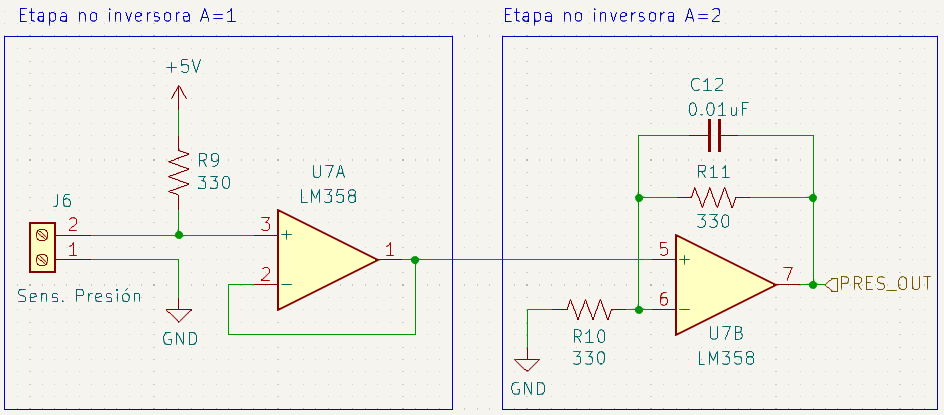
\includegraphics[width=.9\textwidth]{./Figures/circuito-presion.png}
\caption{Diagrama del circuito amplificador de presión.}
\label{fig:circuito-presion}
\end{figure}

\subsection{Factor Lambda}

La señal de salida del LM9044 tiene un rango de 0 a 5 V por lo que tiene que ser reducida a 3,3 V para ser leída por el ADC de la EDU-CIAA. Por eso la salida del integrado es conectada a una etapa seguidora de tensión y luego es atenuada por un divisor resistivo por un factor de 0,6. El circuito está diagramado en la figura \ref{fig:circuito-o2}. Con esta atenuación, para factores lambda de 0,8, 1 y 2, se tiene una señal de salida de, 2,16 V, 1,215 V y 0V. Con estos valores se cumple el rango requerido por REQ-ADQ-004.

\begin{figure}[htpb]
\centering
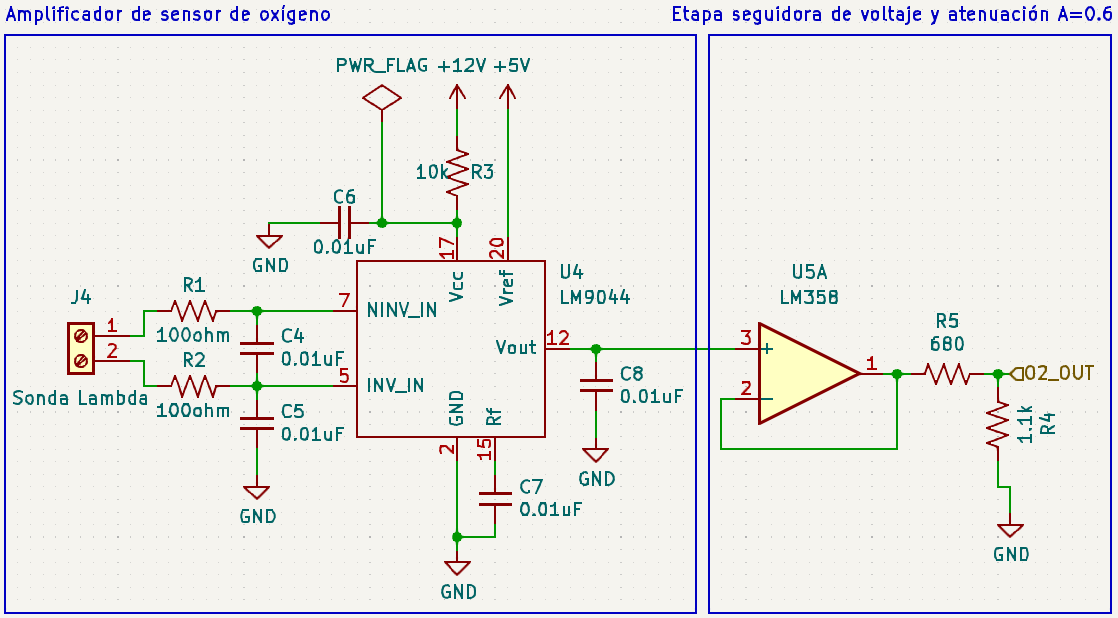
\includegraphics[width=\textwidth]{./Figures/ampli-o2.png}
\caption{Diagrama del circuito amplificador de la sonda lambda.}
\label{fig:circuito-o2}
\end{figure}

\subsection{Tensión de batería}

La medición de la tensión de batería no es un requisito del proyecto. Sin embargo, durante el desarrollo del circuito, surgió la idea de incluir esta medición ya que la información sería de gran utilidad a la hora de ensayar el funcionamiento del circuito.
Las baterías de plomo y ácido tienen una tensión nominal de 12 V, a circuito abierto su tensión entre bornes es de 14,7 V y cuando están completamente descargadas su tensión es de 10,5 V.

La batería alimenta a todo el circuito, su tensión es disminuida a 5 V por un regulador de voltaje LM7805 para alimentar a todos los circuitos integrados que requieren una alimentación de 5 V, como los amplificadores operacionales, el amplificador de sonda lambda y la EDU-CIAA misma. Luego, la salida del regulador de 3,3 V interno de la EDU-CIAA es utilizada para alimentar el resto de los circuitos integrados que operan con 3,3 V, como los circuitos de lectura de termocupla y la interfaz para el sensor de R.P.M.

Para leer la tensión de batería con el ADC de la EDU-CIAA, esta tiene que ser reducida a un valor máximo de 3,3 V. Esto se logró con un divisor resistivo y a su salida un amplificador de ganancia 1 V/V, visto en la figura \ref{fig:circuito-bat} . La función del amplificador es para que la impedancia del ADC no afecte a la tensión de salida del divisor resistivo.

\begin{figure}[htpb]
\centering
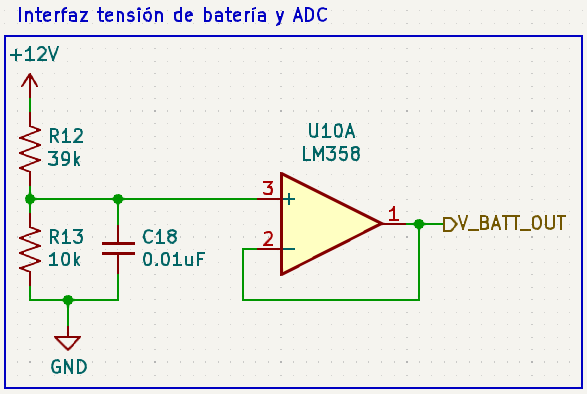
\includegraphics[width=.7\textwidth]{./Figures/ampli-bat.png}
\caption{Diagrama del circuito de reducción de tensión de la batería.}
\label{fig:circuito-bat}
\end{figure}

Con los valores de resistencia seleccionados, una tensión de batería de 16,2 V en la entrada del ADC será de 3,3 V. Y la resolución de la medición será de 0,016 V.

\break

\section{Desarrollo del firmware}

El firmware desarrollado para la parte adquisidora se escribió en el lenguaje de programación C y está implementado sobre FreeRTOS. El empleo de FreeRTOS como un sistema de tiempo real determinista, brinda beneficios significativos al trabajar con sensores. Proporciona una plataforma sólida y confiable para la adquisición y procesamiento de datos en tiempo real. La arquitectura elegida para el desarrollo del firmware es la de "Segmentación de proceso". En donde los procesos productores son las tareas que digitalizan los sensores, el proceso de buffer está implementado en una cola, y el proceso consumidor es la tarea que consulta si hay mensajes disponibles en la cola, los toma, y los envía por el puerto serie al módulo \textit{Bluetooth}.

En total, el firmware tiene que digitalizar las señales de siete sensores, tres termocuplas, sonda lambda, presión de aceite, tensión de batería y el sensor de R.P.M. Para evitar excesivos cambios de contexto por el sistema operativo, se agruparon estas funciones en tres tareas. Una tarea para digitalizar los tres sensores de temperatura llamada \textit{temp-task}, otra para digitalizar los sensores analógicos llamada \textit{analog-task} y la última tarea llamada \textit{rpm-task} digitaliza la señal del sensor de R.P.M. El funcionamiento general del firmware está representado por el diagrama de bloques de la figura \ref{fig:diagrama-firmware}.

\begin{figure}[htpb]
\centering
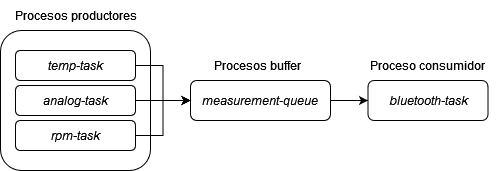
\includegraphics[width=.8\textwidth]{./Figures/diagrama-firmware.png}
\caption{Representación en diagrama de bloques del funcionamiento general del firmware.}
\label{fig:diagrama-firmware}
\end{figure}

El principio de funcionamiento de los procesos productores muy similar para las tres tareas. Primero corren por única vez la rutina de inicialización del sensor, ejecutan la tarea de adquisición de datos, convierten el dato en una variable física, la almacenan en un tipo de dato llamado \textit{measurement} que es almacenado en la cola, y finalmente esperan por un tiempo según la frecuencia de muestreo de ese grupo de sensores. Finalizado ese tiempo se vuelve a repetir el ciclo.

Se desarrolló un módulo de software para lograr la comunicación entre la EDU-CIAA y el integrado MAX31855. La tarea de medición de temperatura, llama una vez por segundo Este integrado integrado digitaliza la señal de termocuplas tipo K en un rango entre -200 \degree C y 700 \degree C con una resolución de 0,25 \degree C. Tiene una interfaz SPI de solo lectura, y una velocidad máxima de muestreo de 1 kHz. Además de informar la lectura de temperatura, también comunica códigos de error si la termocupla esta desconectada, o en cortocircuito con la alimentación o masa \cite{MAX31855}. Con estas características, se cumplen los requisitos REQ-ADQ-001 y REQ-ADQ-002.

Para la rutina de conversión de los sensores analógicos, se utilizaron \textit{lookup tables} para evitar realizar cálculos matemáticos, que pueden ser costosos hablando en tiempo de ejecución. Sobretodo si el sensor no tiene una función lineal, en donde el cálculo puede ser complejo. Como es el caso para la sonda lambda, su función transferencia de factor lambda vs tensión del sensor, está representada en la figura \ref{fig:funcion-lambda}.

\begin{figure}[htpb]
\centering
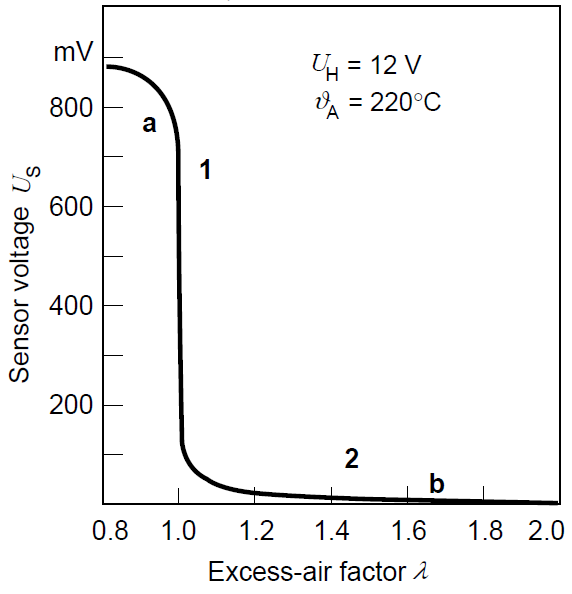
\includegraphics[width=.55\textwidth]{./Figures/funcion-lambda.png}
\caption{Ejemplo de una función transferencia de una sonda Lambda \protect\footnotemark[3].}
\label{fig:funcion-lambda}
\end{figure}
\footnotetext[3]{Imagen tomada de \cite{sondalambda}}

Para la medición de R.P.M. se utilizó el periférico \textit{Timer}, para contar la cantidad de períodos de la señal cuadrada producida por el MAX9924. El \textit{Timer} se configuró para generar interrupciones por flanco positivo y contar cuantos flancos positivos se detectaron en un período de 180 ms. Para el caso de una rueda con un solo diente se genera un pulso por revolución. La resolución de esta forma de lectura es de 333 R.P.M. El rango máximo de medición, depende de la velocidad en la que el sistema pueda atender la interrupción. Que para el caso de 20.000 R.P.M., 60 pulsos en 180 ms, dicha capacidad es suficiente. De esta forma se cumple con el requisito REQ-ADQ-003.

El tipo \textit{measurement} es una estructura de cinco elementos:

\begin{itemize}
\item{\textit{ticks}:} variable de tipo \textit{TickType} definido por FreeRTOS, representa la cantidad de tiempo transcurrida de iniciado el programa en milisegundos.
\item{\textit{value}:} valor de la medición representado como número entero.
\item{\textit{decimal pos}:} posición de la coma decimal.
\item{\textit{name}:} \textit{String} de 4 caracteres de largo que almacena el nombre del sensor.
\item{\textit{fault code}:} número sin signo de 8 bits que puede almacenar códigos de error, solo si es soportado por el sensor.
\end{itemize}

La tarea \textit{bluetooth-task}, convierte al tipo de dato \textit{measurement}, en un arreglo de caracteres o \textit{String} para poder enviarlo por el puerto serie al módulo \textit{HM-10}. Para convertir este tipo de dato a \textit{String} y pueda ser comprendido por el software receptor de datos, se utilizaron los caracteres especiales de la tabla ASCII, \textit{Start of text}, \textit{End of text} y \textit{Group separator}. Que están en las posiciones 2, 3 y 19, de dicha tabla ASCII respectivamente. El caracter \textit{Group separator} sirve para indicar la separación entre dos elementos de la estructura. Los caracteres \textit{Start of text} y \textit{End of text} indican cuando inicia y termina una medición. La estructura convertida a tipo \textit{String} puede verse representada en la figura \ref{fig:measurement-string}. El uso de caracteres especiales requiere enviar una mínima cantidad de \textit{bytes} extra por cada paquete, pero permite que los campos tengan longitudes flexibles y puedan ser diferenciados de forma sencilla. Para que un paquete sea decodificado por la parte receptora, sólo es necesario respetar el orden en el que se envían los campos.

\begin{figure}[htpb]
\centering

\includegraphics[width=.9\textwidth]{./Figures/measurement-string.png}
\caption{La estructura \textit{measurement} convertida a tipo \textit{String}.}
\label{fig:measurement-string}
\end{figure}


\section{Desarrollo de la interfaz gráfica}

Se eligió Python 3.7 como lenguaje de programación para desarrollar el software de la interfaz gráfica. Principalmente porque los scripts desarrollados en Python pueden correr en una gran variedad de dispositivos y en distintos sistemas operativos. Se utilizó el framework gráfico multi-plataforma \textit{Kivy} para la interfaz gráfica en sí. La librería \textit{Matplotlib} para dibujar las gráficas de los sensores. Y a la librería \textit{Bleak} para resolver la comunicación \textit{Bluetooth} entre las partes del dispositivo. La figura \ref{fig:gui} muestra el resultado final de la interfaz gráfica.

El principal desafío al desarrollar la interfaz gráfica fue la decodificación de la información recibida por \textit{Bluetooth}. El problema es los datos recibidos llegan en paquetes de longitud variable, que no necesariamente encapsulan a un único \textit{measurement} convertido a \textit{String}. Por esto, se implementó una máquina de estados que al recibir un paquete de datos, busca los caracteres \textit{Start of text} y \textit{End of text}. Al recibir un \textit{Start of text}, la máquina de estados concatena los datos recibidos hasta que encuentra un \textit{End of text} que indica el final de un \textit{measurement}. Una vez que se recibió un \textit{measurement} completo, es almacenado en una \textit{dataclass} de Python que contiene los elementos: \textit{ticks}, \textit{value}, \textit{decimal pos}, \textit{name} y \textit{fault code}. Esta clase es equivalente a la estructura utilizada en el firmware de la parte adquisidora.

Nuevamente la arquitectura utilizada fue la de "Segmentación de proceso". En este caso, el proceso productor es una tarea que resuelve la recepción de datos por \textit{Bluetooth}, los decodifica a través de dicha máquina de estados, y almacena a cada tipo de medición en una cola FIFO. Otra tarea asincrónica actúa como proceso consumidor, y dibuja en pantalla la información recibida en sus gráficas correspondientes. Además, esta tarea responde a las acciones del usuario.

\begin{figure}[htpb]
\centering
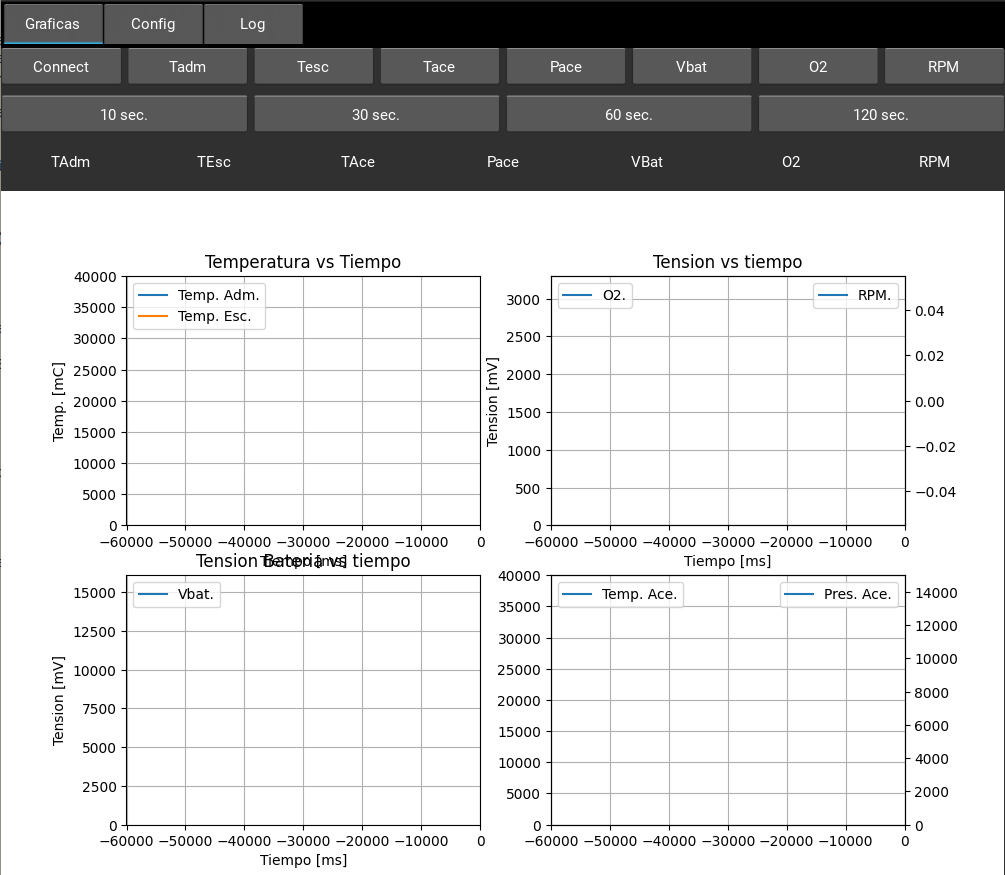
\includegraphics[width=.9\textwidth]{./Figures/gui.png}
\caption{Captura de pantalla del resultado final de la interfaz gráfica.}
\label{fig:gui}
\end{figure}


\chapter{Ensayos y resultados}

\label{Chapter4}

En este capítulo se describen los ensayos llevados a cabo para verificar que todos los requisitos del proyecto fueron cumplidos.

\section{Ensayos de verificación}

Se ensambló un banco de ensayos para poder evaluar el rendimiento del sistema y resolver los fallos que se experimentaron durante el desarrollo. De esta forma, se evitó la dependencia de disponer un motor de combustión interna para los ensayos. Las figuras \ref{fig:banco-pruebas-1} y \ref{fig:banco-pruebas-2} muestran dicho banco de pruebas durante uno de ellos.

\begin{figure}[htpb]
\centering
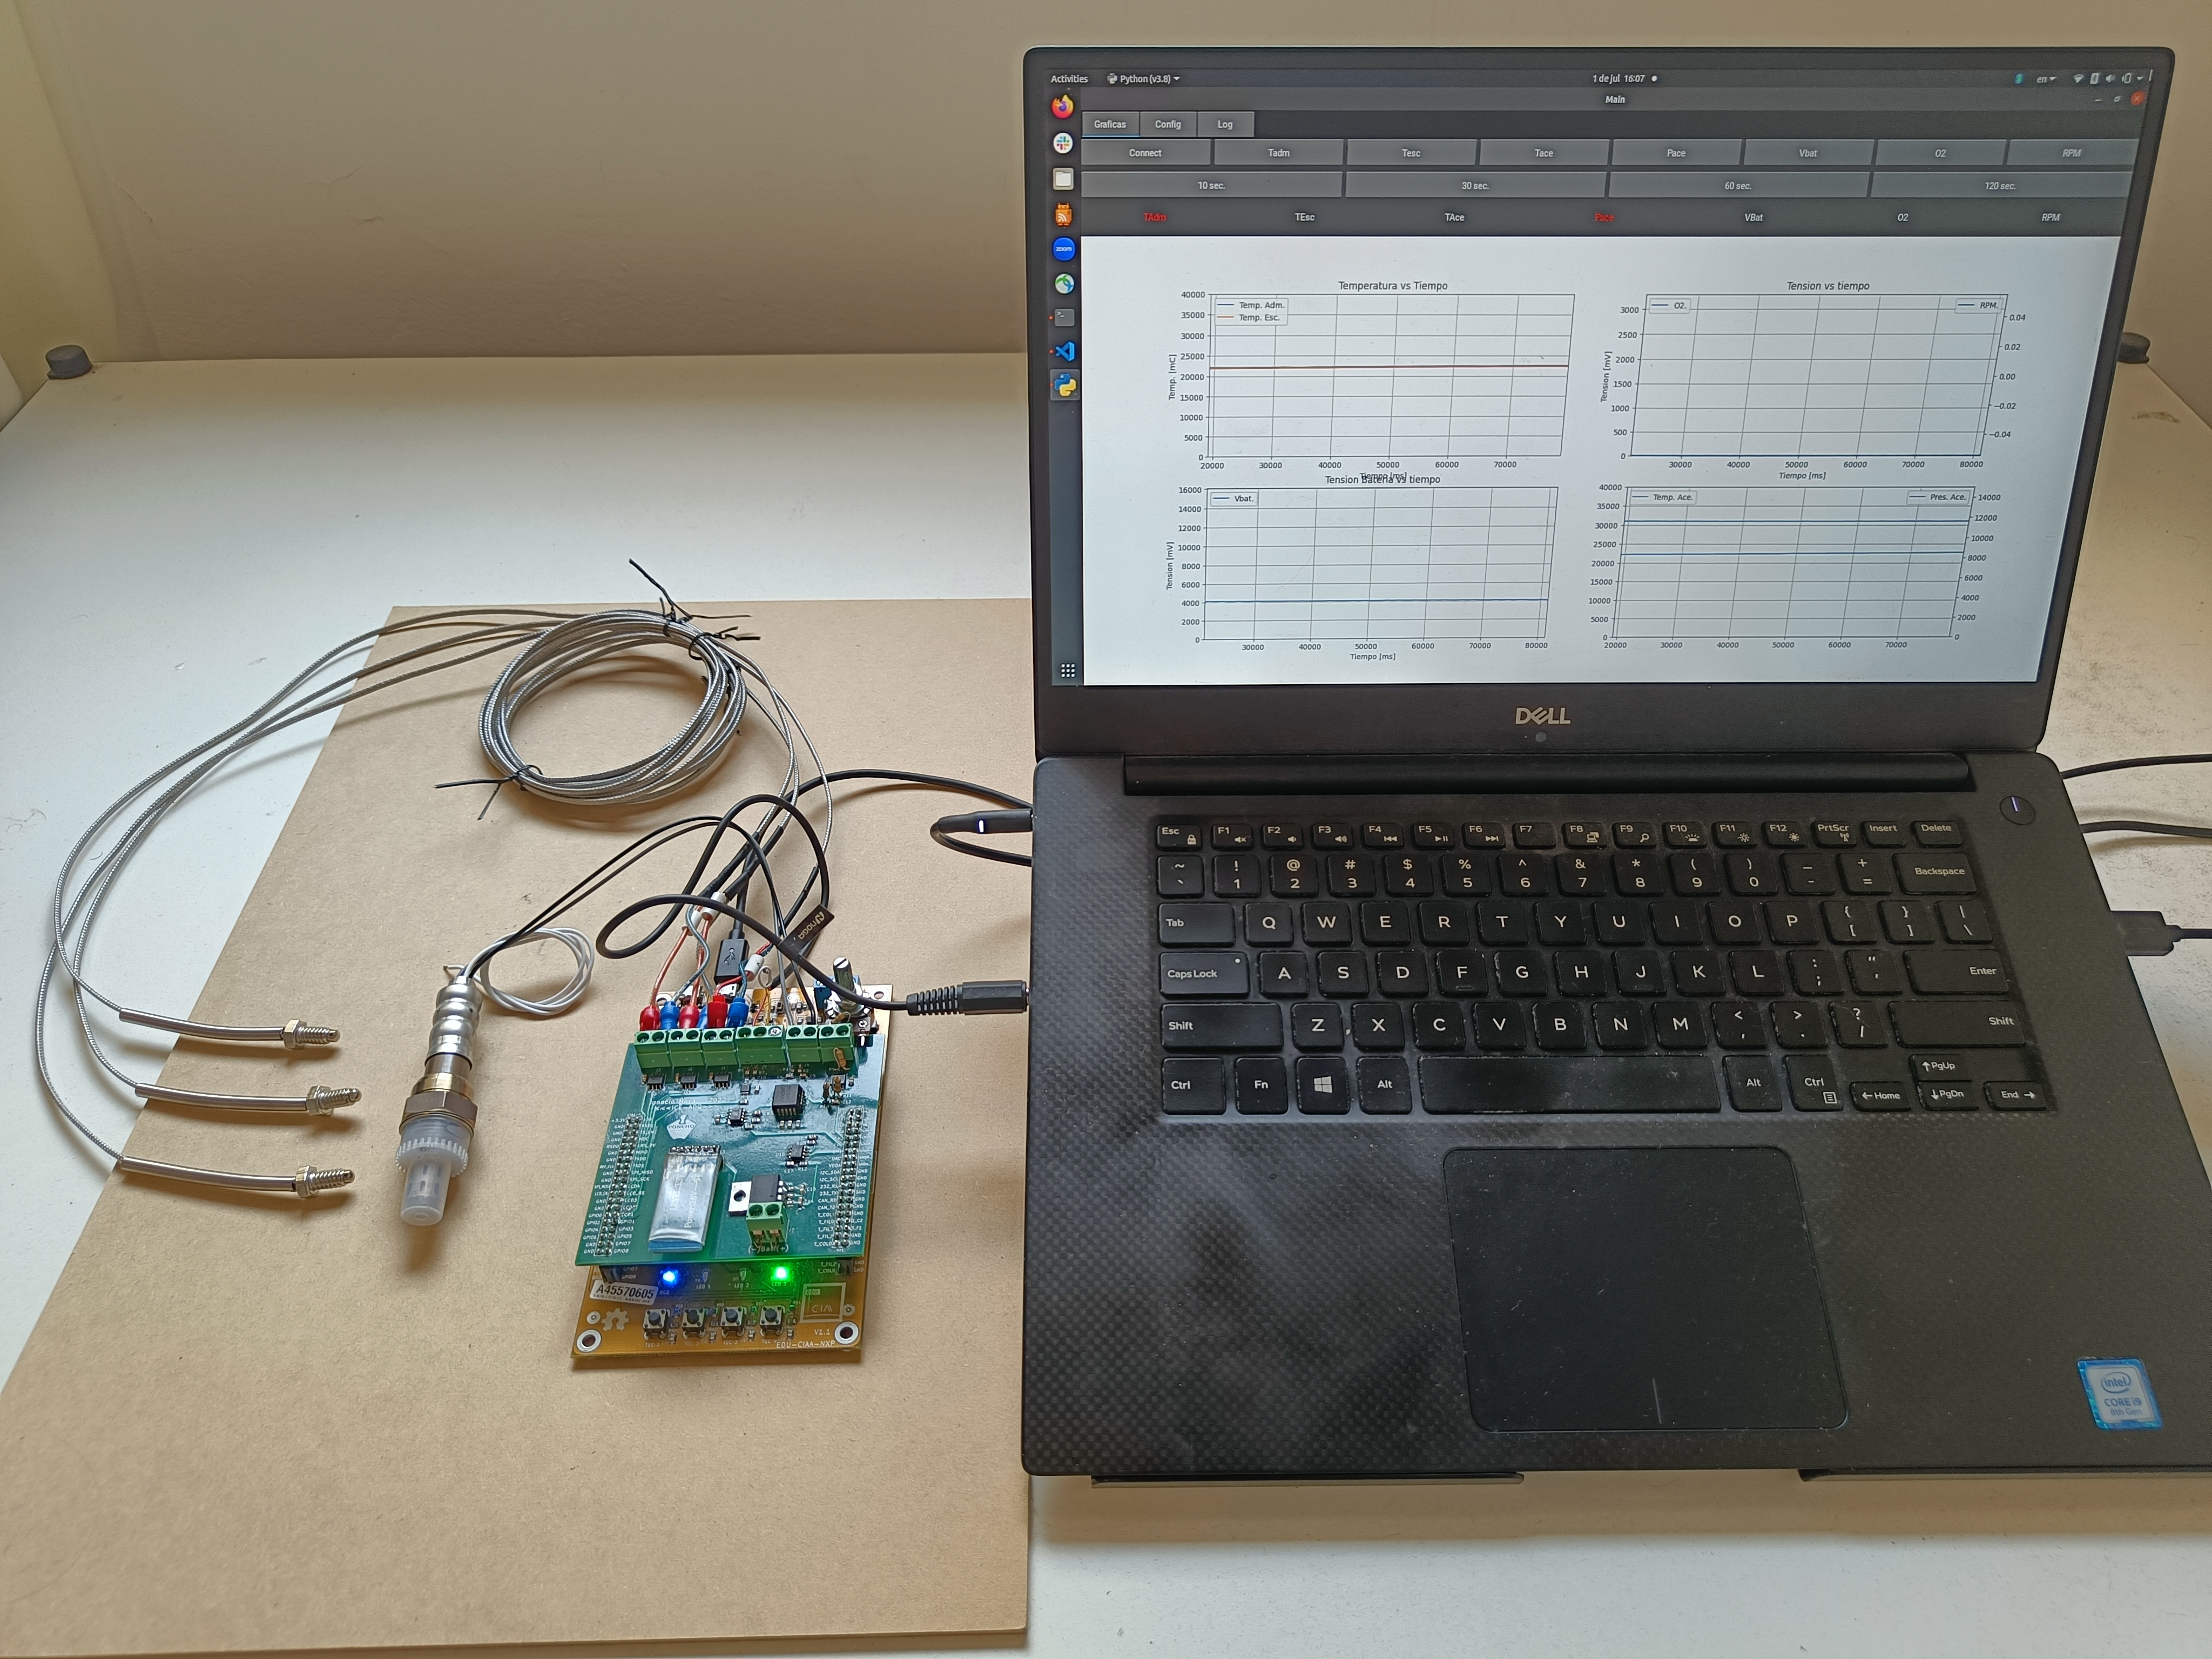
\includegraphics[width=.85\textwidth]{./Figures/banco-pruebas-1.jpg}
\caption{Fotografía del banco de pruebas durante uno de los ensayos.}
\label{fig:banco-pruebas-1}
\end{figure}

\begin{figure}[htpb]
\centering
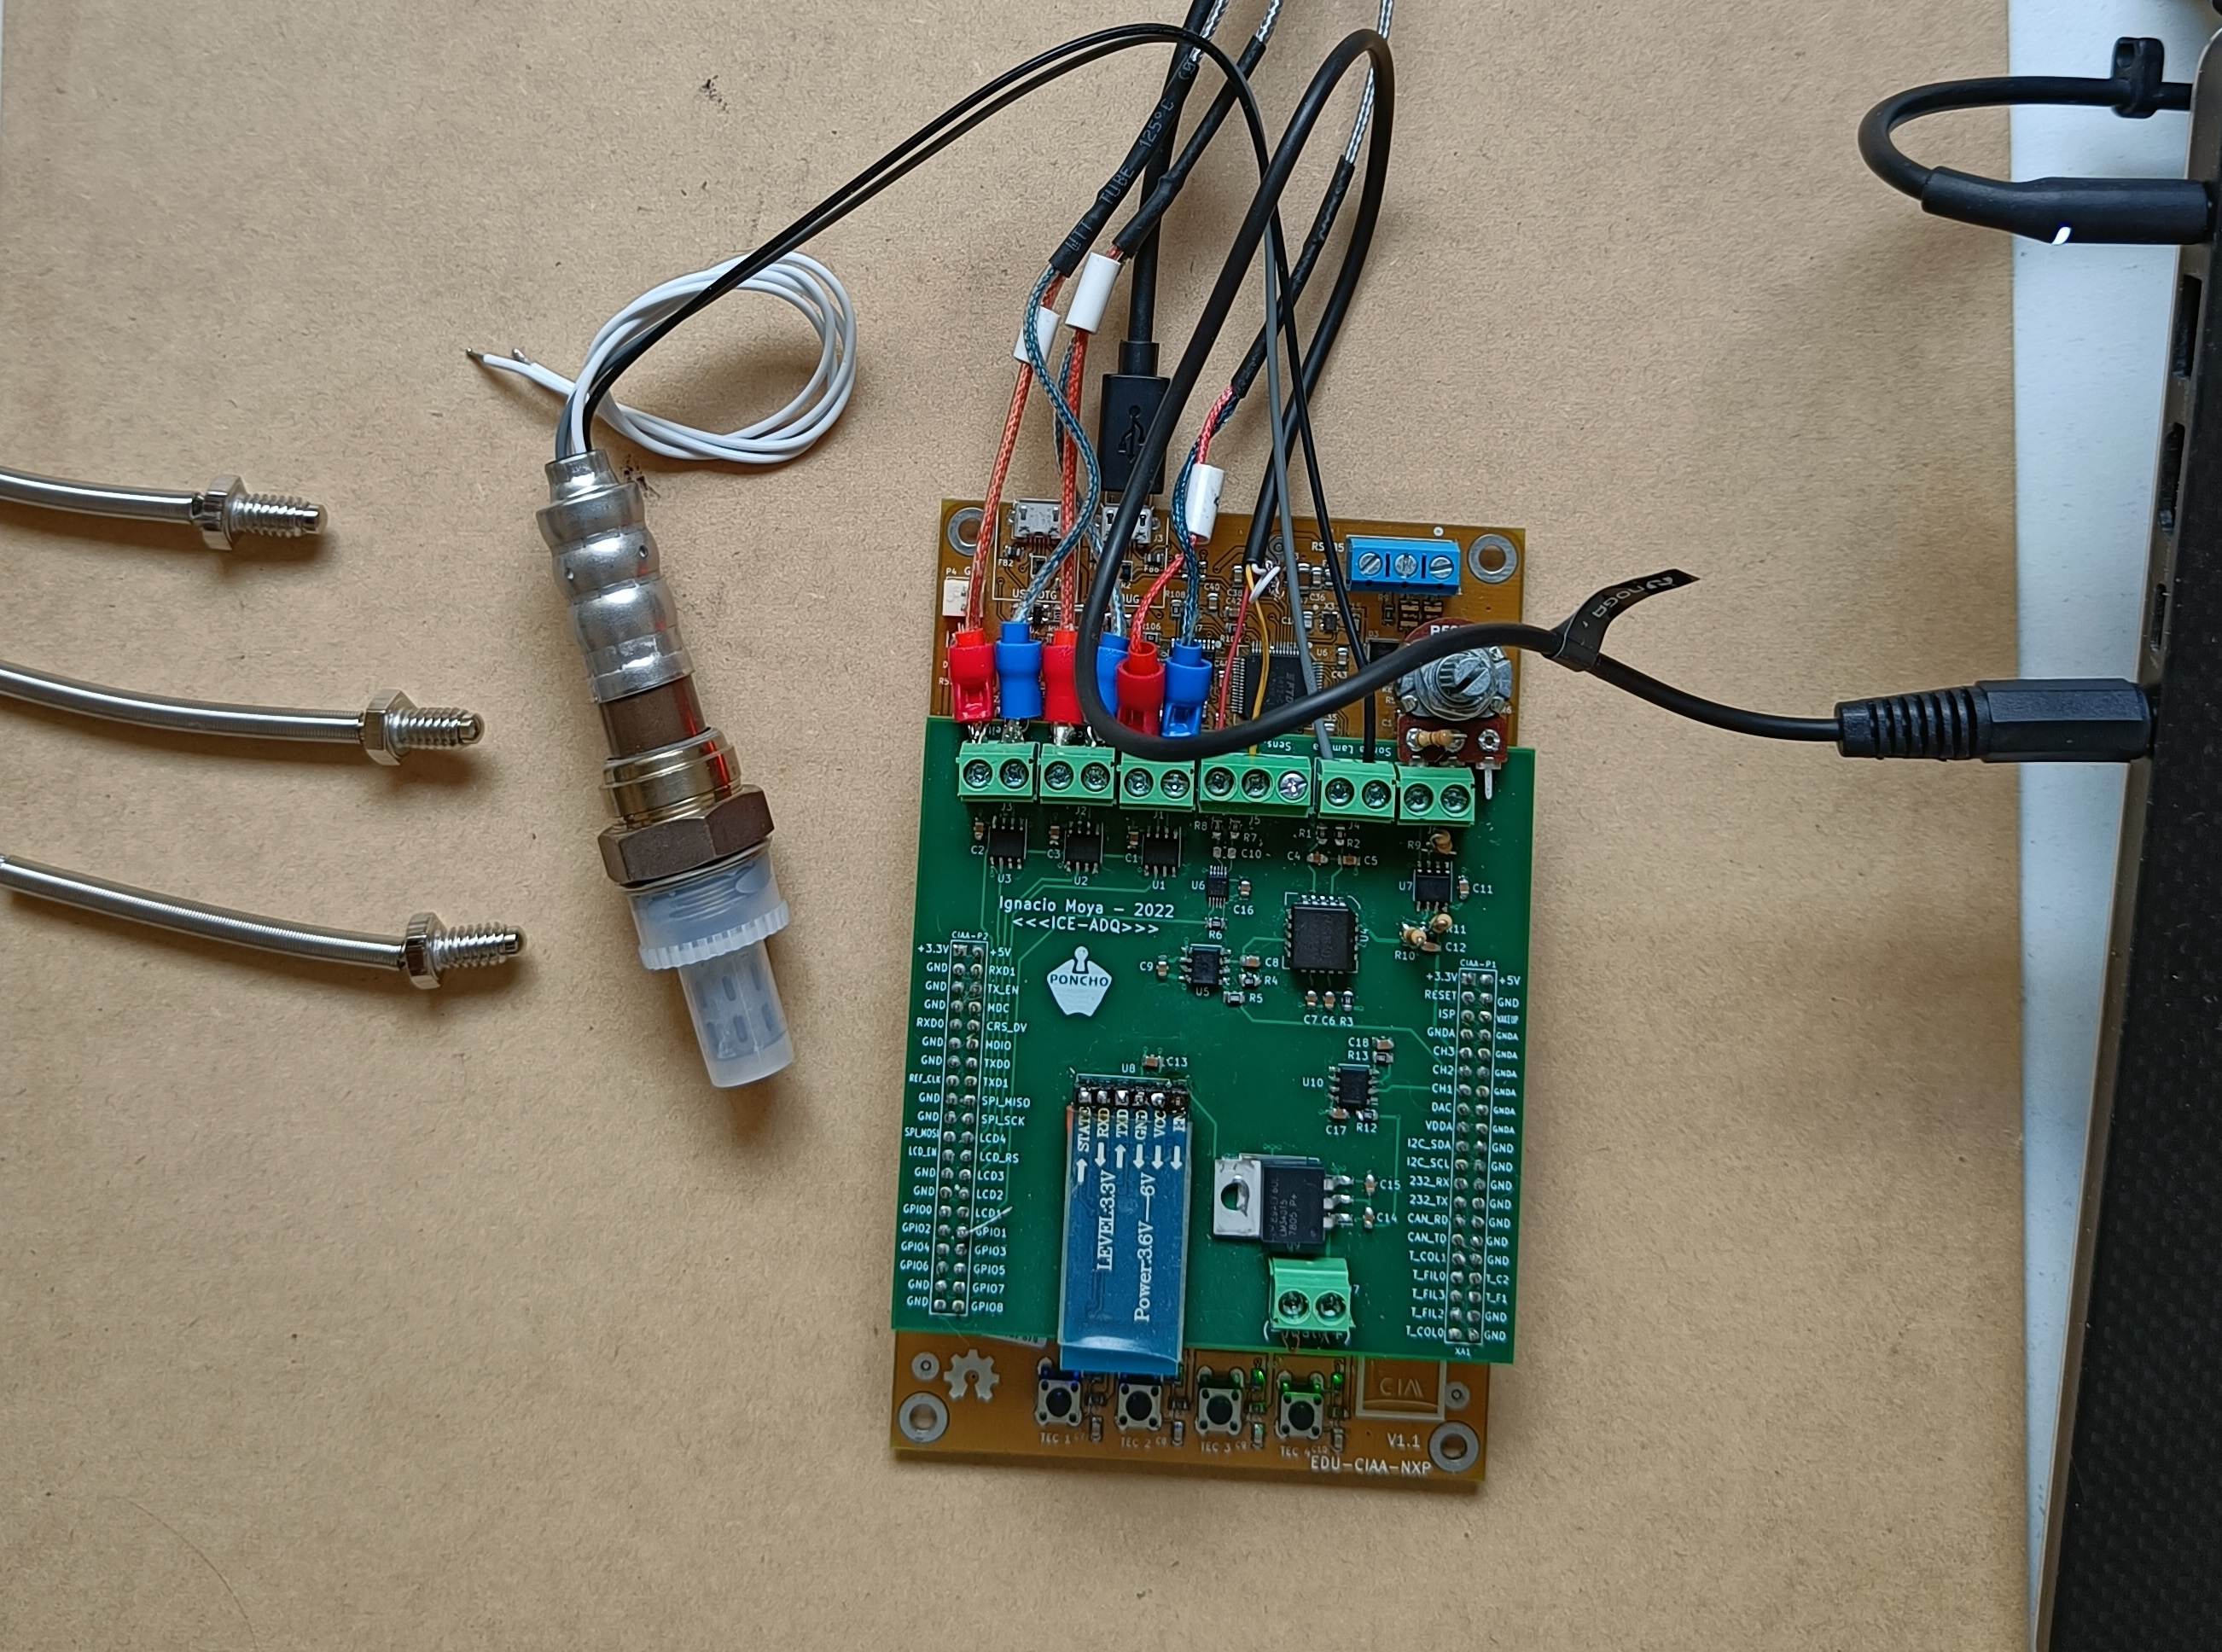
\includegraphics[width=.85\textwidth]{./Figures/banco-pruebas-2.jpg}
\caption{Fotografía en detalle del circuito impreso montado sobre la EDU-CIAA y con sensores conectados.}
\label{fig:banco-pruebas-2}
\end{figure}
\break
\subsection{Ensayos de medición de temperatura}

Se contrastaron las mediciones realizadas por el sistema contra las mediciones realizadas por un multímetro, que incluye la opción para medir temperatura a través de termocuplas tipo K. Las termocuplas se sumergieron en un recipiente con agua y se repitió el ensayo tres veces, en los que se utilizaron temperaturas de referencias 0 \degree C, 20 \degree C (considerada temperatura ambiente) y 80 \degree C. Para cada ensayo a distinta temperatura se tomaron 150 muestras consecutivas, que representan un tiempo total transcurrido de 375 segundos o 6 minutos 15 segundos. Luego, para cada juego de muestras se calculó su valor medio y la desviación estandar, para lograr cuantificar el error y la dispersión que tuvieron las medidas de temperatura tomadas por el sistema. Estos resultados están plasmados en las figuras \ref{fig:temp-0c}, \ref{fig:temp-20c} y \ref{fig:temp-80c}.

\begin{figure}[htpb]
\centering
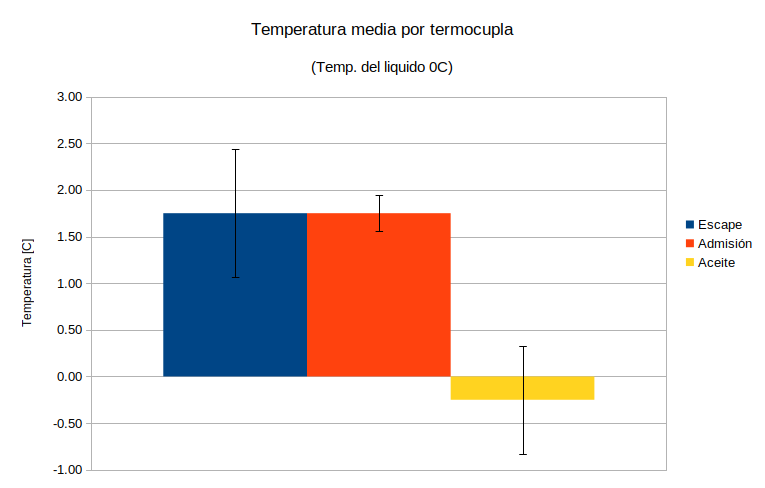
\includegraphics[width=.9\textwidth]{./Figures/temp-0c.png}
\caption{Valores medios y desviación estándar para el ensayo de temperatura a 0 \degree C.}
\label{fig:temp-0c}
\end{figure}

\begin{figure}[htpb]
\centering
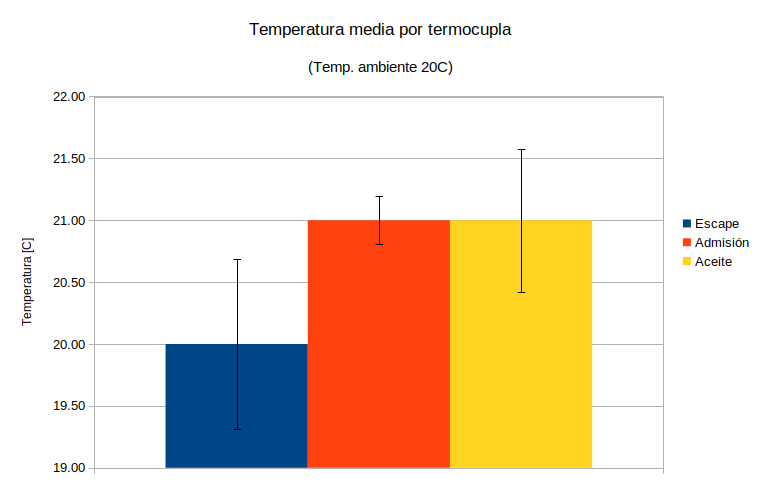
\includegraphics[width=.9\textwidth]{./Figures/temp-20c.png}
\caption{Valores medios y desviación estándar para el ensayo de temperatura a 20 \degree C.}
\label{fig:temp-20c}
\end{figure}

\begin{figure}[htpb]
\centering
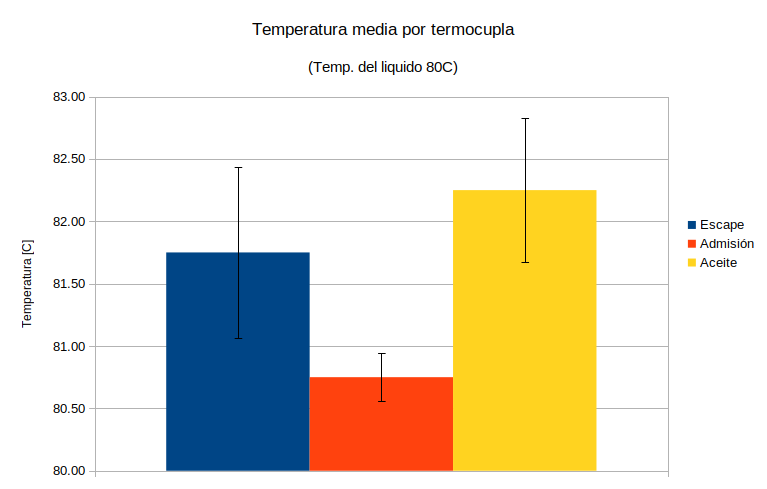
\includegraphics[width=.9\textwidth]{./Figures/temp-80c.png}
\caption{Valores medios y desviación estándar para el ensayo de temperatura a 0 \degree C.}
\label{fig:temp-80c}
\end{figure}

El resultado con menor diferencia al valor contrastado fue para la termocupla de temperatura de aceite en el ensayo de 0 \degree C, dicho error fue de 0,25 \degree C. La mayor diferencia se encontró para la termocupla de aceite en el ensayo a 80 \degree C, en ese caso el error fue de 2,25 \degree C. La menor desviación estándar se registró para la termocupla de temperatura de admisión, en el ensayo de 0 \degree C, su valor fue de 0,179 \degree C. La mayor desviación estándar se registró para la termocupla de temperatura de aceite en el ensayo de 80 \degree C, su valor fue de 0,806 \degree C.  Los valores de error y desviación máximos registrados son considerados aceptables.

\break

\subsection{Ensayos de medición de velocidad de giro}

Para este ensayo se desarrolló, con una placa de desarrollo Arduino "MEGA", un simulador de una señal proveniente de un sensor de reluctancia variable. El objetivo de este programa es generar una señal cuadrada periódica, de frecuencia seleccionable, y de ciclo de trabajo positivo de 10\%.

Para verificar la medición del sistema, se realizaron ocho mediciones de la señal simulada a distintos valores de R.P.M. Para contrastar los resultados obtenidos se utilizó un osciloscopio digital como instrumento de medición de calidad. Dichos resultados están plasmados en la tabla \ref{tab:ensayo-rpm}. En la figura \ref{fig:foto-rpm} se aprecia ambas placas conectadas entre si, y la forma de onda de la señal generada (en amarillo), y la señal producida por el MAX9924 (en azul) en la pantalla del osciloscopio.

\begin{figure}[htpb]
\centering
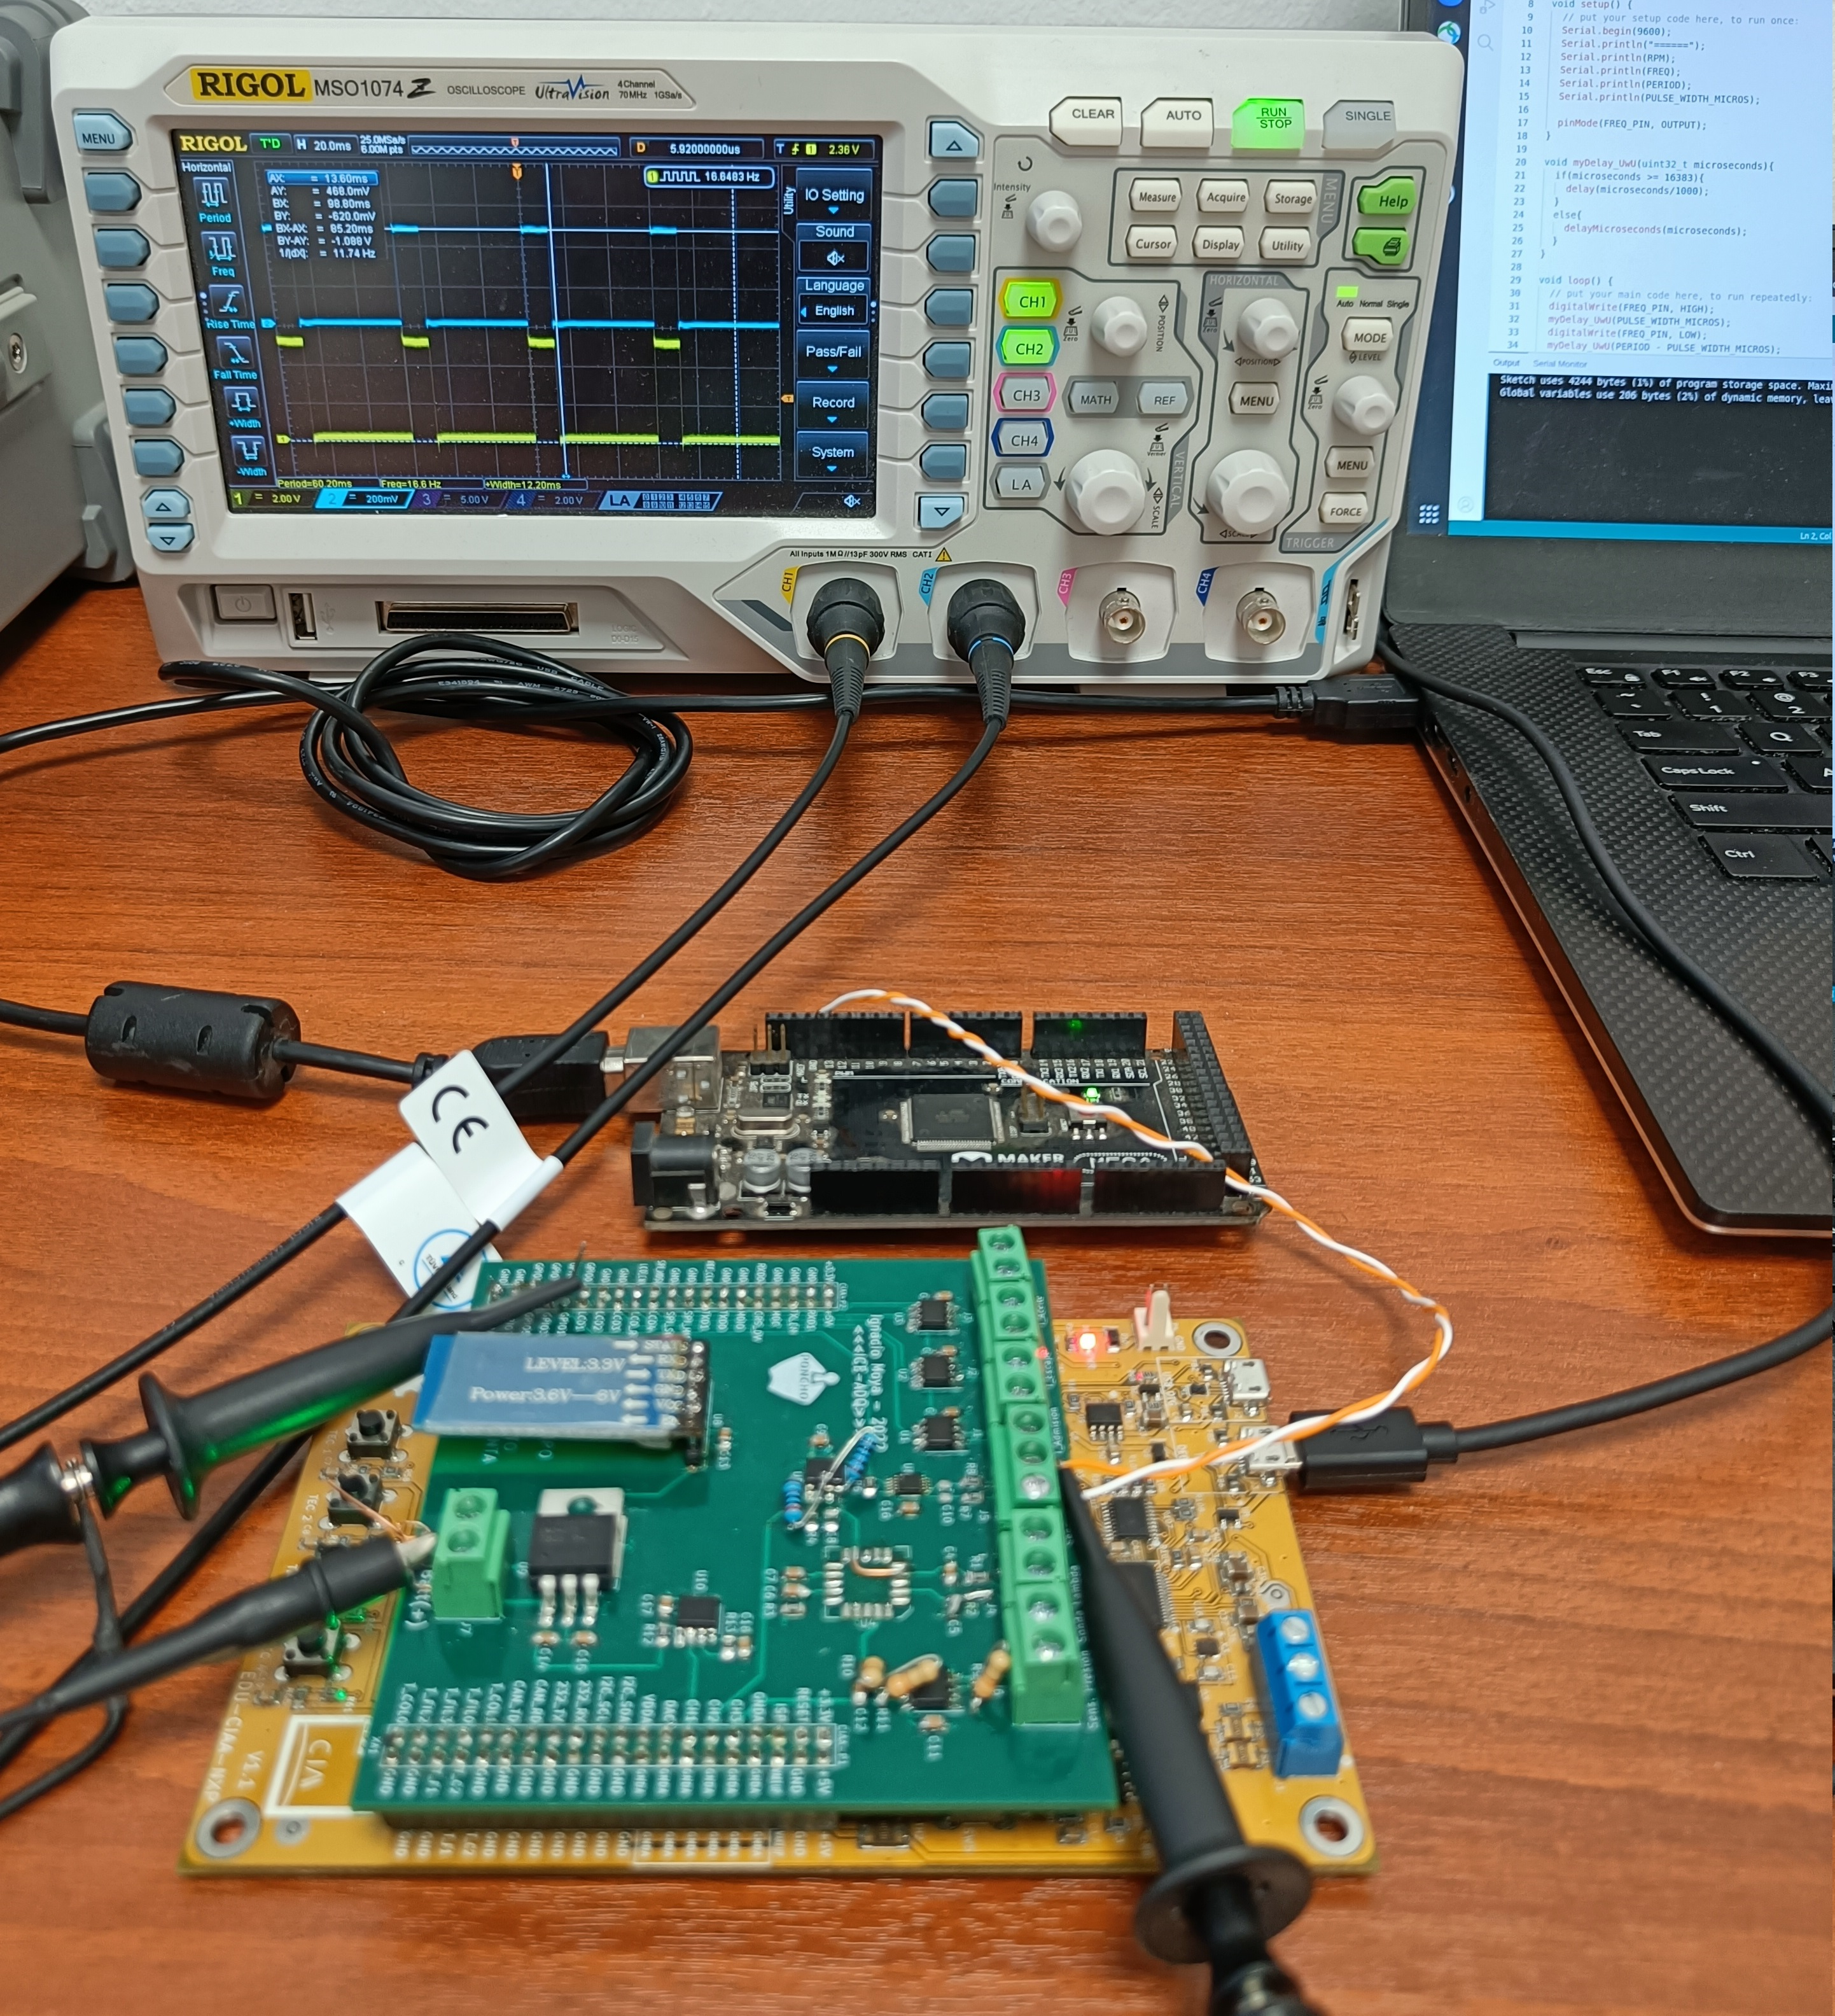
\includegraphics[width=.8\textwidth]{./Figures/foto-rpm.jpg}
\caption{Foto del sistema en funcionamiento conectado a la placa Arduino "MEGA" utilizada como simulador de señal de R.P.M.}
\label{fig:foto-rpm}
\end{figure}

\begin{table}[htpb]
	\centering
	\caption{Resultados de ensayo de medición de velocidad de giro.}
	\centering
	\begin{tabular}{c c c c}    
		\toprule
		\textbf{Simulada[RPM]} &  \textbf{Referencia[RPM]}   & \textbf{Observada[RPM]} & \textbf{Error[RPM]}\\
		\midrule
		1000	&	998 &	900 & 98\\
		2500	&	2577 & 2400 & 177\\
		5000	&	4967 & 5100 & -133 \\
		7500	&	7447 & 7500 & -53\\
		10000	&	9925 & 9900 & 25\\
		12500	&	12402 & 12300 & 102\\
		15000	&	14876 & 14700 & 176\\
		17500	&	17182 & 17100 & 82\\
		20000	&	19817 & 19800 & 17\\		
		\bottomrule
	\end{tabular}
	\label{tab:ensayo-rpm}
\end{table}

Como se puede observar de los resultados del ensayo. La diferencia máxima entre el valor medido y el contrastado fue de 133 R.P.M., con esto entonces se cumple con el requisito REQ-ADQ-003.

\break

\subsection{Ensayos de medición de presión de aceite}

Para verificar que la medición de presión de aceite cumpliera con el requisito REQ-ADQ-005 se realizaron dos ensayos distintos.

En el primero se simuló al sensor de presión con un potenciómetro de valor similar. Luego se midió la tensión en los contactos de la bornera en donde se conecta el sensor con el circuito impreso. Y, finalmente, se contrastó el valor de tensión medido, con la lectura realizada por el ADC, para observar en cuanto diferían entre sí. Los resultados del ensayo están listados en la tabla \ref{tab:ensayo-presion}. El error máximo se dio para el caso de 0,847 V, equivalente a una presión de 66,007 PSI y fue de 0,519 PSI. Dicho error es considerado aceptable. 

\begin{table}[htpb]
	\centering
	\caption{Resultados de ensayo medición de presión de aceite.}
	\centering
	\begin{tabular}{c c c c}    
		\toprule
		\textbf{Tensión[V]} & \textbf{Presión equivalente[PSI]} & \textbf{Lectura[PSI]} & \textbf{Error[PSI]}\\
		\midrule
		0,172		&   5,980 & 5,580 & 0,4 \\
		0,847		&   66,007 & 65,488 & 0,519 \\
		1,429		&   117,764 & 117,418 & 0,346 \\
		\bottomrule
	\end{tabular}
	\label{tab:ensayo-presion}
\end{table}

\subsection{Ensayos de medición de la sonda lambda}

Ante la falta de un dispositivo capaz de leer una sonda lamba para luego contrastar su lectura. Se simuló una sonda Lambda con una fuente de tensión variable digital. Y se realizaron mediciones para 11 valores de tensión, de forma de simular distintos valores de factor lambda. Los resultados del ensayo pueden verse en la tabla \ref{tab:ensayo-o2}. El error máximo registrado fue de 0.019, considerado aceptable para la aplicación.

\begin{table}[htpb]
	\centering
	\caption{Resultados de ensayo medición de factor lambda.}
	\centering
	\begin{tabular}{c c c c}    
		\toprule
		\textbf{Tensión[V]} & \textbf{Lambda equivalente[$\lambda$]} & \textbf{Lectura[$\lambda$]} & \textbf{Error[$\lambda$]} \\
		\midrule
		0		&	2	 & 1.946 & 0.054 \\		
		0,1		&   1,26 & 1.316 & -0.056 \\
		0,2		&   1,06 & 1.089 & -0.029 \\
		0,3		&   1.04 & 1.035 & 0.005 \\
		0,45	&   1 	 & 1 	 & 0 \\
		0,5		&   0.98 & 0.971- & 0.009 \\
		0,6		&   0.92 & 0.924 & -0.004 \\
		0,7		&   0.88 & 0.872 & 0.008 \\
		0,8		&   0.84 & 0.843 & -0.003 \\
		0,9		&   0.65 & 0.656 & -0.006 \\
		1		&   0	 & 0.019 & -0.019 \\
		\bottomrule
	\end{tabular}
	\label{tab:ensayo-o2}
\end{table}

\subsection{Ensayo de pérdida de paquetes}

Para este ensayo se modificó el software de ambas partes del sistema para agregar un campo extra a cada paquete transmitido. Cada uno de ellos fue enumerado con una cifra que comienza en 0 y se incrementa en 1 cada vez que se transmite un paquete. De esta forma, es posible saber si existieron pérdidas de paquetes durante la transmisión, luego de verificar que la secuencia de los números no se vio interrumpida al finalizar el ensayo. Luego, se colocaron ambas partes separadas por una distancia de tres metros y se inició la trasmisión de información hasta llegar a la cantidad de 10.000 paquetes transmitidos.

Resultado: No se encontró pérdida de datos después de 10.000 transmisiones consecutivas, se verificó que el requisito REQ-COMM-001 fue cumplido con éxito.

\subsection{Ensayo de tiempo de transmisión}

En esta prueba, para poder emplear los dos pines de propósito general disponibles, se modificó el firmware. Uno de ellos se utilizó para indicar, con un nivel lógico alto, que la tarea de medición de temperatura está en proceso de adquisición. El pin restante se utilizó para indicar cuando el paquete measurement fue envíado por la tarea de transmisión. Entonces, a través de un analizador lógico, se midió el tiempo entre los cambios de estado de ambos pines. De esta forma, fue posible medir el tiempo que transcurrió entre que se obtiene una medición de la variable, hasta que es transmitida. El resultado de una de estas mediciones puede apreciarse en la figura \ref{fig:tiempo-envio}. El tiempo promedio, luego de tomar diez mediciones consecutivas, fue de 52,2 ms. De esta forma se cumple con el requisito REQ-ADQ-006.

\begin{figure}[htpb]
\centering
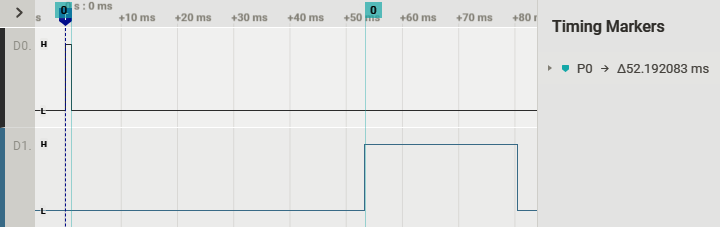
\includegraphics[width=\textwidth]{./Figures/tiempo-envio.png}
\caption{Captura de pantalla del software del analizador lógico, donde se puede apreciar que el tiempo que transcurre entre, adquisición y envío del dato, es de 52 ms aproximadamente.}
\label{fig:tiempo-envio}
\end{figure}

\section{Casos de uso}

En esta sección se describen los casos de uso y las pruebas realizadas para validar, si la interfaz gráfica cumple con sus requerimientos de aceptación. Al mismo tiempo, se utilizaron estos ensayos para evaluar si son necesarios cambios o mejoras en el diseño de la interfaz. Los casos de uso están descriptos en las tablas  \ref{tab:caso-conectar}, \ref{tab:caso-ocultar}, \ref{tab:caso-mostrar}, \ref{tab:caso-aumentar}, y \ref{tab:caso-decrementar}.

Al finalizar estas pruebas, se verificó que el diseño y la implementación de la interfaz gráfica son adecuados para cumplir con sus requisitos. Sin embargo, se encontró que la pantalla utilizada era de un tamaño muy pequeño, y esto dificulta la lectura de las gráficas y la interacción con los botones a través de la interfaz táctil.

\begin{table}[htpb]
	\centering
	\caption{Caso de uso: conectarse a la parte adquisidora.}
	\centering
	\begin{tabular}{c p{0.6\textwidth}}    
		\toprule
		\textbf{Título }     & \textbf{Descripción} \\
		\midrule
		Identificador		&  CU1. \\
		Nombre				&   Conectarse a parte adquisidora. \\
		Actor principal		&   Usuario \\
		Disparadores		&   El usuario presiona el botón \textit{Conectar} \\
		Flujo básico		&   \\
		Pre-condiciones		&   La parte adquisidora tiene que estar en funcionamiento y su LED azul parpadeando. \\
		Post-condiciones	&    \\
		\bottomrule
	\end{tabular}
\label{tab:caso-conectar}
\end{table}

\begin{table}[htpb]
	\centering
	\caption{Caso de uso: ocultar una variable de su gráfica.}
	\centering
	\begin{tabular}{c p{0.6\textwidth}}    
		\toprule
		\textbf{Título }     & \textbf{Descripción} \\
		\midrule
		Identificador		&  CU2. \\
		Nombre				&   Ocultar variable en la gráfica. \\
		Actor principal		&   Usuario \\
		Disparadores		&   El usuario presiona el botón que tiene el mismo nombre de la variable que quiere ocultar. \\
\\
		Pre-condiciones		&   La variable se encuentra visible. \\
		Post-condiciones	&   La variable deja de estar visible.\\
		\bottomrule
	\end{tabular}
\label{tab:caso-ocultar}
\end{table}

\begin{table}[htpb]
	\centering
	\caption{Caso de uso: mostrar una variable oculta.}
	\centering
	\begin{tabular}{c p{0.6\textwidth}}    
		\toprule
		\textbf{Título }     & \textbf{Descripción} \\
		\midrule
		Identificador		&	CU3. \\
		Nombre				& 	Mostrar variable oculta. \\
		Actor principal		&   Usuario \\
		Disparadores		&   El usuario presiona el botón que tiene el mismo nombre de la variable que quiere mostrar. \\
\\
		Pre-condiciones		&   La variable se encuentra oculta. \\
		Post-condiciones	&   La variable es visualizada en su gráfica correspondiente.\\
		\bottomrule
	\end{tabular}
\label{tab:caso-mostrar}
\end{table}

\begin{table}[htpb]
	\centering
	\caption{Caso de uso: aumentar valor de alarma.}
	\centering
	\begin{tabular}{c p{0.6\textwidth}}    
		\toprule
		\textbf{Título }     & \textbf{Descripción} \\
		\midrule
		Identificador		&	CU4. \\
		Nombre				& 	Aumentar valor de alarma. \\
		Actor principal		&   Usuario \\
		Disparadores		&   El usuario presiona alguno de los botones + que se encuentran al lado de los nombres de las variables. \\
\\
		Pre-condiciones		&   Ninguna \\
		Post-condiciones	&   El valor de la alarma se incrementa en una unidad.\\
		\bottomrule
	\end{tabular}
\label{tab:caso-aumentar}
\end{table}

\begin{table}[t!]
	\centering
	\caption{Caso de uso: disminuir valor de alarma.}
	\centering
	\begin{tabular}{c p{0.6\textwidth}}    
		\toprule
		\textbf{Título }     & \textbf{Descripción} \\
		\midrule
		Identificador		&	CU5. \\
		Nombre				& 	Disminuir valor de alarma. \\
		Actor principal		&   Usuario \\
		Disparadores		&   El usuario presiona alguno de los botones - que se encuentran al lado de los nombres de las variables. \\
\\
		Pre-condiciones		&   Ninguna \\
		Post-condiciones	&   El valor de la alarma disminuye por una unidad.\\
		\bottomrule
	\end{tabular}
\label{tab:caso-decrementar}
\end{table}

 
\chapter{Conclusiones}

\label{Chapter5}

Al finalizar del trabajo, se demostró que fue posible desarrollar y fabricar un prototipo, que cumpla con todos los requisitos planteados durante la fase de planificación del proyecto. En el transcurso tuvieron que superarse desafíos y resolver problemas. Como por ejemplo, la selección de reemplazo de componentes que estaban en falta, y el desarrollo de una interfaz gráfica de usuario sin experiencia previa. Gracias a eso se logró obtener suficiente conocimiento y experiencia para poder continuar con el trabajo, y aplicarlo para avanzar del prototipo a un producto final.

\section{Trabajo futuro}
Con el objetivo de continuar el desarrollo para llegar a un dispositivo final que pueda ser comerciable, se identificó que se debe continuar trabajando en los siguientes ítems:

\begin{itemize}
\item Durante la etapa de ensayos fue muy difícil leer la información desde la pantalla LCD de 5 pulgadas, la interfaz gráfica deberá ser optimizada para que pueda ser empleada en pantallas de tamaños reducidos.

\item Para poder proteger a la parte adquisidora de las condiciones que existen dentro del habitáculo del motor, se tendrá que desarrollar o seleccionar un gabinete para resguardarla y evitar posibles daños.

\item Reemplazar las borneras con tornillos por conectores aptos para trabajar en condiciones de alta temperatura y vibración.

\item Desarrollar un sistema de montaje para poder anclar al gabinete al habitáculo del motor.

\item Desarrollar un arnés de conexión entre los sensores y el circuito impreso.

\item Mejorar el circuito agregando protecciones contra descargas electroestáticas y radiación electromagnética.

\item Investigar otros métodos de comunicación, especialmente que permitan mayor ancho de banda, para poder aumentar la cantidad de sensores o la tasa de muestreo.

\end{itemize}



 

%----------------------------------------------------------------------------------------
%	CONTENIDO DE LA MEMORIA  - APÉNDICES
%----------------------------------------------------------------------------------------

\appendix % indicativo para indicarle a LaTeX los siguientes "capítulos" son apéndices

% Incluir los apéndices de la memoria como archivos separadas desde la carpeta Appendices
% Descomentar las líneas a medida que se escriben los apéndices

%% Appendix A

\chapter{Appendix Title Here} % Main appendix title

\label{AppendixA} % For referencing this appendix elsewhere, use \ref{AppendixA}

Write your Appendix content here.
1%\include{Appendices/AppendixB}
%\include{Appendices/AppendixC}

%----------------------------------------------------------------------------------------
%	BIBLIOGRAPHY
%----------------------------------------------------------------------------------------

\Urlmuskip=0mu plus 1mu\relax
\raggedright
\printbibliography[heading=bibintoc]

%----------------------------------------------------------------------------------------

\end{document}  
